\chapter{IBM Rational DOORS}
\label{chap:kapitel3}

Rational DOORS ist ein Anforderungsmanagement-Tool des US-amerikanischen IT-Unternehmens IBM. Das Akronym \acs{DOORS} steht für Dynamic Object-Oriented Requirements System \cite[]{q5}.
Dieses Tool wird zur Dokumentation und Verwaltung von Anforderungen genutzt. Die \acs{DOORS} Datenbank ist dabei hierarchisch aufgebaut und besteht aus drei verschiedenen Elementen, nämlich den 
Projekten, den Ordnern und den Modulen. Dieser Aufbau ist in Abbildung \ref*{fig:Doors GUI} zu erkennen. Projekte und Ordner werden dafür genutzt, um die Daten innerhalb der \acs{DOORS} Datenbank 
zu organisieren und zu strukturieren. Projekte sind in der GUI erkennbar durch ein blaues Ordner-Symbol, während Ordner durch ein gelbes Ordner-Symbol gekennzeichnet werden. Dies kann ebenfalls der 
Abbildung \ref*{fig:Doors GUI} entnommen werden. Projekte und Ordner unterscheiden sich vorallem dadurch, dass die Namen von Projekten in der gesamten Datenbank eindeutig sein müssen. 
Die Position aller Daten innerhalb eines Projekts ist durch den Pfad, welcher mit dem Projekt beginnt, festgelegt \cite[]{q6}. Die Funktionsweise von Ordnern hingegen, ist vergleichbar 
zu den Ordnern im Windows Explorer.     

\begin{figure}[H]
    \centering
    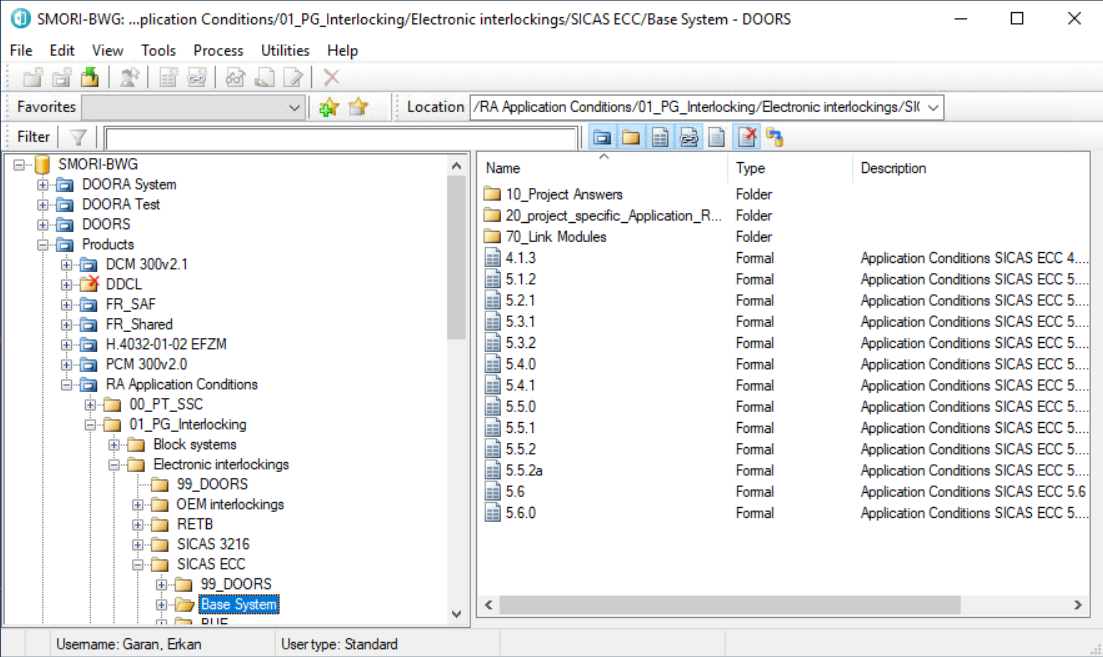
\includegraphics[width = \textwidth]{abbildungen/IBM Doors.PNG}
    \caption{GUI der \acs{DOORS} Anwendung}
    \label{fig:Doors GUI}
\end{figure}

Die Module in \acs{DOORS} sind die Elemente, welche die Anforderungen in einer tabellarischen Form beinhalten. Abbildung \ref*{fig:Doors Modul} zeigt ein geöffnetes Modul in \acs{DOORS}. Dort ist zu erkennen,
dass die einzelnen Spalten die Attribute darstellen, die einzelnen Zeilen werden dabei Objekte genannt. Zudem hat der User die Möglichkeit oben links neben dem Feld \glqq View\grqq{} eine View auszuwählen. Mithilfe einer View 
ist der User in der Lage durch Filter, Sortierungen, Ein- bzw. Ausblenden von Spalten u.Ä. sich nur das anzeigen zu lassen, was für ihn aktuell relevant ist. Rechts neben dem Text des Objekts sind 
zwei verschiedene Pfeile zu erkennen. Diese Pfeile zeigen an, dass Links, also Verbindungen von oder zu diesem Objekt bestehen. Links sind essentiell für das Requirements Tracing, also für die
Verfolgung von Anforderungen. Dadurch wird deutlich von wo eine Anforderung herkommt oder wo sie ebenfalls genutzt wird. Der rote Pfeil mit der Spitze nach rechts ist dabei ein Out-Link, also eine
Verbindung von dem Objekt zu einem anderen Objekt. Der gelbe Pfeil mit der Spitze in die entgegengesetzte Richtung symbolisiert einen In-Link, also eine Verbindung von einem anderen Objekt zu diesem 
Objekt. Eine weitere Form von Modulen sind die Link-Module. Diese werden dafür verwendet, um Informationen über Links zu speichern. 

\begin{figure}[H]
    \centering
    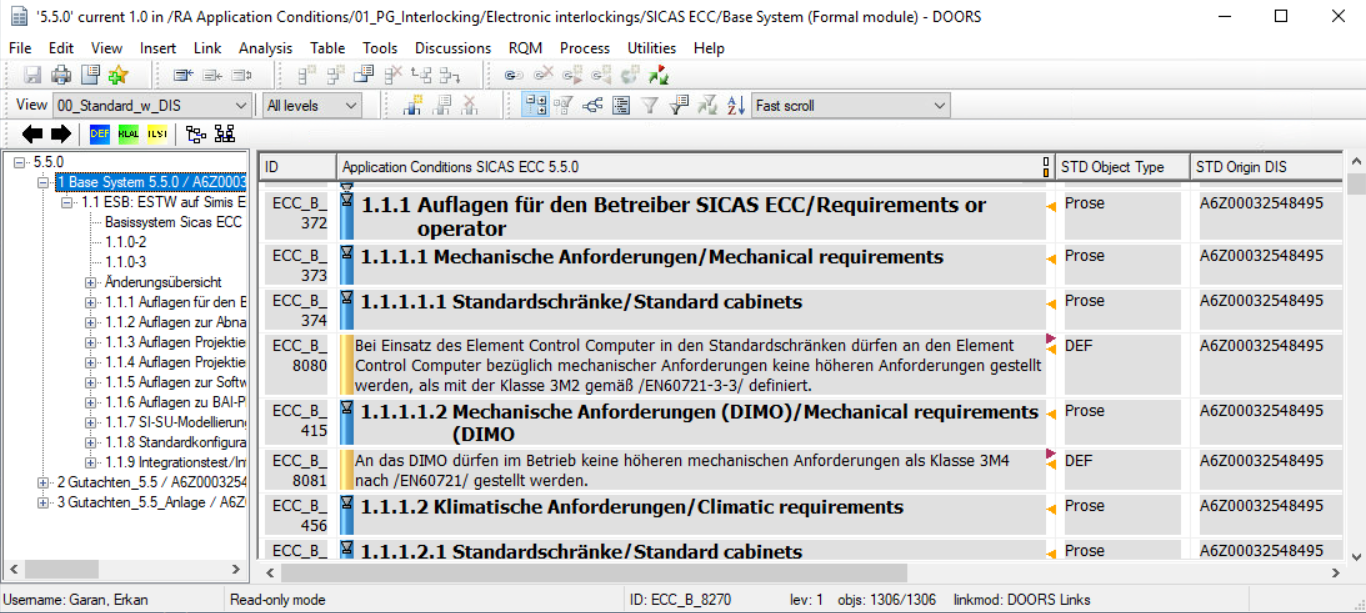
\includegraphics[width = \textwidth]{abbildungen/Modul in Doors.PNG}
    \caption{Modul in \acs{DOORS}}
    \label{fig:Doors Modul}
\end{figure}

Neben der Arbeit mittels der grafischen Benutzeroberfläche bietet die \ac*{DXL} eine weitere Möglichkeit um mit \acs{DOORS} zu arbeiten. \acs{DXL} ist dabei eine Scripting-Sprache, deren
Syntax der von C und C++ ähnelt und dafür genutzt werden kann, um Skripte zu erstellen. Mit diesen Skripten können beispielsweise Module oder Ordner erstellt werden, sowie Objekte angelegt und 
editiert werden \cite[]{q7}. 